\chapter{Introdução}
\label{cap:introducao}

A engenharia de software passa atualmente por uma profunda transformação com a transição dos Modelos de Linguagem de Larga Escala (\textit{Large Language Models} - LLMs) de interfaces conversacionais passivas para agentes autônomos orientados a objetivos. Diferente do modelo tradicional de perguntas e respostas pontuais, esses agentes operam em ciclos contínuos de raciocínio, planejamento e ação. Eles dividem metas complexas em etapas menores, definem parâmetros de execução e acionam rotinas em ambientes computacionais distribuídos \cite{buhler2026agentbound,singh2026mcpsecure}.

Para interagir com o mundo real e superar as limitações de seus dados de treinamento estáticos, os agentes de IA dependem do mecanismo de chamada de ferramentas (\textit{tool calling}) e do acesso a dados contextuais externos. Essas fontes incluem bancos de dados relacionais, sistemas de arquivos locais, repositórios de código e interfaces de programação de aplicações (APIs) \cite{zhu2025miniscope,hasan2026mcp}. No entanto, a integração entre modelos de linguagem e ferramentas externas sempre sofreu com a fragmentação técnica: cada plataforma adotava conectores proprietários e soluções pontuais, gerando forte acoplamento, problemas de compatibilidade e políticas de segurança frágeis ou inconsistentes.

Para resolver essa fragmentação, a Anthropic lançou no final de 2024 o \textit{Model Context Protocol} (MCP), uma arquitetura aberta de comunicação cliente-servidor baseada no protocolo JSON-RPC 2.0. O MCP rapidamente se consolidou como o padrão da indústria para conectar aplicações que hospedam modelos de IA (\textit{MCP Hosts/Clients}) a fontes de dados e ferramentas de execução (\textit{MCP Servers}) \cite{soriaparra2026mcp,hasan2026mcp}. Ao padronizar três conceitos fundamentais: ferramentas executáveis (\textit{tools}), dados e arquivos de leitura (\textit{resources}) e modelos de instrução (\textit{prompts}), o MCP permitiu que uma mesma aplicação cliente se conecte a dezenas de servidores locais (via canais de comunicação interprocessos \textit{stdio}) ou remotos (inicialmente via SSE e atualmente via \textit{Streamable HTTP}) \cite{soriaparra2026mcp}.


\begin{figure}[H]
  \centering
  \caption{Arquitetura de Integração do Model Context Protocol.}
  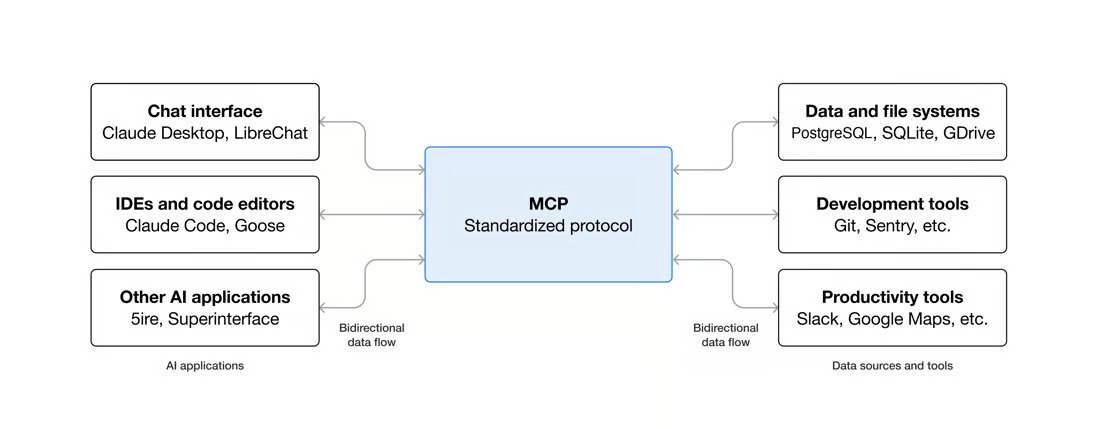
\includegraphics[scale=0.4]{mcp-official-anthropic-diagram.jpg}
  \label{fig:integration-arch}
  \caption*{Fonte: Anthropic (2024)}
\end{figure}

Apesar da facilidade de integração oferecida pelo protocolo, pesquisas recentes mostram que essa rápida expansão introduziu uma superfície de ataque ampla e preocupante no ecossistema de software \cite{guo2025measurement,hou2025mcp}. O MCP foi concebido sob uma postura estrutural de \textbf{confiança implícita}: uma vez realizada a conexão inicial entre o cliente e o servidor, o agente passa a ter acesso aberto a todas as ferramentas expostas, executando ações no sistema operacional com os mesmos privilégios do usuário logado \cite{buhler2026agentbound,singh2026mcpsecure}.

Estudos recentes de medição em larga escala comprovam a gravidade desse cenário. Em uma análise empírica de 1.899 servidores MCP de código aberto, Hasan et al. \cite{hasan2026mcp} identificaram que o protocolo apresenta uma superfície dual de ataque: além de 7,2\% dos servidores conterem falhas clássicas no código-fonte (com credenciais e chaves de acesso gravadas em texto simples em 3,6\% dos projetos), 5,5\% dos servidores já sofrem de envenenamento de ferramentas (\textit{Tool Poisoning}). Nesse tipo de ataque, descrições e esquemas das ferramentas são alterados de forma maliciosa para induzir o modelo de linguagem a tomar decisões incorretas ou prejudiciais, sem que o código executável precise ser modificado. Além disso, Guo et al. \cite{guo2025measurement} demonstraram que mais de 50\% dos servidores MCP em uso executam chamadas sensíveis no sistema hospedeiro (como execução de comandos de shell, leitura de arquivos e conexões de rede irrestritas) sem qualquer mecanismo de isolamento de processos.

Conforme analisado por Jang e Lee \cite{jang2026hierarchical}, o protocolo MCP funciona como um canal de integração que herda riscos de segurança em três camadas diferentes: na camada da própria LLM (injeções indiretas de prompt e alucinações), na camada do protocolo (ataques de intermediação maliciosa como \textit{Confused Deputy} e \textit{Puppet Attacks}) e na camada de infraestrutura de rede (envenenamento de DNS e ataques de atualização fraudulenta conhecidos como \textit{Rug Pull}, como o incidente registrado no servidor \texttt{postmark-mcp}).

Por outro lado, Bühler et al. \cite{buhler2026agentbound} destacaram a existência da \textbf{lacuna semântica} (\textit{Semantic Gap}) na segurança de agentes de IA: mecanismos tradicionais de isolamento do sistema operacional (como contêineres e políticas de controle de acesso de kernel) são essenciais para conter danos ao hospedeiro, mas não conseguem avaliar a intenção do agente nem impedir o uso indevido de ferramentas que tenham sido autorizadas no sistema. Ao mesmo tempo, Zhang et al. \cite{zhang2025acfix} comprovaram que confiar decisões de acesso à saída probabilística de modelos de linguagem gera falhas de quebra de controle de acesso (\textit{Broken Access Control}) em 47,4\% dos casos, reforçando a necessidade de aplicar modelos determinísticos de Controle de Acesso Baseado em Papéis (\textit{Role-Based Access Control} - RBAC).

Diante desse cenário, percebe-se a falta de uma solução unificada que combine a aplicação prática do Princípio do Menor Privilégio (\textit{Principle of Least Privilege}) em tempo de execução, a geração de registros de auditoria forense confiáveis e a observabilidade detalhada do tráfego de mensagens do protocolo. É exatamente nesse espaço de pesquisa que este trabalho se desenvolve.

% -----------------------------------------------------------------------------
% MOTIVAÇÃO
% -----------------------------------------------------------------------------
\section{Motivação}
\label{sec:motivacao}

O avanço rápido das tecnologias baseadas em modelos de linguagem fez com que os agentes autônomos deixassem de ser apenas experimentos de laboratório e passassem a ser integrados diretamente a processos produtivos e corporativos. Em empresas de tecnologia, finanças, atendimento ao cliente e desenvolvimento de software, esses agentes já são empregados para automatizar tarefas complexas, como consultar e atualizar bancos de dados, gerar e aplicar modificações em repositórios de código, acionar rotinas de integração contínua e interagir com serviços em nuvem.

Nesse ecossistema em expansão, o Model Context Protocol (MCP) assumiu um papel central como a principal especificação de integração, sendo rapidamente adotado por grandes plataformas de desenvolvimento, ambientes integrados (IDEs) e clientes de IA. Essa ampla aceitação deve-se à simplicidade e à conveniência com que o protocolo permite que desenvolvedores disponibilizem dados e ferramentas para modelos inteligentes.

Entretanto, essa rápida popularização gerou um descompasso preocupante: priorizou-se a velocidade de conexão e a facilidade de uso, enquanto os mecanismos de controle, governança e segurança foram deixados em segundo plano. Na prática, quando um agente de IA recebe acesso a um servidor MCP em um ambiente corporativo, ele frequentemente passa a operar com permissões excessivas, capazes de causar prejuízos operacionais graves caso o modelo interprete instruções incorretas, sofra manipulações maliciosas ou alucine durante a execução.

Além dos riscos operacionais diretos, como a exclusão acidental de arquivos ou a alteração indevida de registros em bancos de dados, a ausência de mecanismos rigorosos de controle expõe as organizações a sérios riscos regulatórios. Normas de proteção de dados (como a LGPD no Brasil e a GDPR na União Europeia) e padrões de segurança da informação exigem que qualquer acesso a informações sensíveis seja rigorosamente controlado, registrado e auditável. Quando uma organização não consegue comprovar quem autorizou uma ação, quais ferramentas foram executadas por um agente e se os registros de log foram alterados, ela fica exposta a penalidades legais, falhas de conformidade e danos à sua reputação.

Portanto, a motivação deste trabalho reside na necessidade urgente de desenvolver soluções práticas e eficientes que permitam às organizações aproveitar a automação e o poder dos agentes de IA baseados em MCP, sem abrir mão da segurança, do controle de acesso e da capacidade de auditar cada ação executada.

% -----------------------------------------------------------------------------
% PROBLEMÁTICA
% -----------------------------------------------------------------------------
\section{Problemática}
\label{sec:problematica}

A especificação técnica oficial do Model Context Protocol \cite{soriaparra2026mcp} padronizou o modelo de transporte e o formato das mensagens JSON-RPC 2.0, mas não incluiu mecanismos nativos de governança ou controle de acesso em tempo de execução. Em vez disso, a especificação delegou as decisões de segurança aos clientes hospedeiros ou à confirmação manual do usuário por meio de janelas de diálogo (\textit{prompts} de aprovação).

Na prática diária, essa abordagem apresenta falhas estruturais graves. Por um lado, depender exclusivamente da confirmação manual do usuário gera fadiga de alertas: diante de dezenas de solicitações contínuas, os usuários tendem a aprovar chamadas sem verificar os parâmetros técnicos detalhados de cada operação. Por outro lado, o modelo de confiança implícita do protocolo permite que, após a conexão inicial, o agente execute qualquer ferramenta disponibilizada pelo servidor. Esse cenário resulta em quatro problemas fundamentais:

\begin{enumerate}
  \item \textbf{Falta de Mediação e Controle em Tempo de Execução:} Inexistência de um ponto de aplicação de políticas (\textit{Policy Enforcement Point} - PEP) que inspecione as mensagens trocadas entre o cliente e o servidor. Quando um agente sofre um desvio de comportamento provocado por uma injeção indireta de prompt inserida em um dado externo não confiável, ele pode acionar ferramentas com efeitos destrutivos (como apagar dados ou sobrescrever arquivos) sem que qualquer regra impeça a execução \cite{singh2026mcpsecure};

  \item \textbf{Ausência de Controle de Acesso Baseado em Papéis (RBAC):} O protocolo expõe ferramentas de leitura e de escrita de forma indiferenciada na mesma sessão de trabalho. Não existe uma separação formal entre operações seguras (como consultas informativas) e operações críticas que alteram o estado do sistema, deixando os ambientes vulneráveis a falhas generalizadas de controle de acesso (\textit{Broken Access Control}) \cite{zhang2025acfix,zhu2025miniscope};

  \item \textbf{Dificuldade de Auditoria Forense e Falta de Garantia de Integridade:} Os servidores MCP geram registros de log heterogêneos, voláteis e desprovidos de proteção criptográfica contra adulteração (\textit{tamper-evident}). Diante de um incidente de segurança ou de uma ação indevida do agente, torna-se praticamente impossível reconstituir com exatidão a cadeia de eventos: qual modelo disparou a ferramenta, com quais argumentos, sob qual contexto e se os registros foram alterados posteriormente;

  \item \textbf{Falta de Visibilidade Operacional e Telemetria em Tempo Real:} Embora a especificação mais recente do MCP sugira a adoção de padrões abertos como o OpenTelemetry \cite{soriaparra2026mcp}, as implementações práticas não dispõem de instrumentação centralizada. Equipes de engenharia e segurança não conseguem visualizar em tempo real as taxas de chamadas, as requisições bloqueadas nem o comportamento de latência das conexões.
\end{enumerate}

Essa problemática é agravada pelo fato de que os mecanismos clássicos de segurança no sistema operacional não entendem o significado das operações solicitadas pelo agente (a chamada \textit{lacuna semântica} descrita por Bühler et al. \cite{buhler2026agentbound}), enquanto delegar o controle de acesso ao próprio modelo de linguagem resulta em decisões falhas e inconsistentes \cite{zhang2025acfix}.

Com base nessas limitações, define-se a seguinte \textbf{Pergunta de Pesquisa (\textit{Research Question})}:

\begin{quote}
  \textit{Como conceber, implementar e validar experimentalmente uma camada intermediária de governança em tempo de execução para ecossistemas baseados no Model Context Protocol (MCP) que aplique controle de acesso baseado no menor privilégio (RBAC), garanta auditabilidade forense imutável e forneça telemetria padronizada, sem exigir alterações no código-fonte dos clientes e servidores existentes, garantindo latência insignificante para sistemas em produção?}
\end{quote}

% -----------------------------------------------------------------------------
% HIPÓTESE DE INVESTIGAÇÃO
% -----------------------------------------------------------------------------
\section{Hipótese de Investigação}
\label{sec:hipotese}

A hipótese científica de trabalho adotada nesta pesquisa afirma que:

\begin{quote}
  \textbf{Hipótese de Trabalho:} \textit{A introdução de uma camada intermediária de governança não invasiva no canal de comunicação JSON-RPC do MCP --- operada por um mecanismo determinístico de Controle de Acesso Baseado em Papéis (RBAC) com divisão clara entre operações de leitura e mutação, combinada com uma trilha de auditoria forense criptografada e um módulo de telemetria compatível com OpenTelemetry --- é capaz de interceptar e bloquear com eficácia vetores de ataque adversariais (como Tool Poisoning, Rug Pull e Broken Access Control) com uma sobrecarga de latência imperceptível ($< 1,0$ ms por chamada), induzindo ao mesmo tempo o efeito de Moldagem Comportamental, que torna as decisões e o planejamento do próprio agente de IA mais seguros.}
\end{quote}

% -----------------------------------------------------------------------------
% OBJETIVOS DA PESQUISA
% -----------------------------------------------------------------------------
\section{Objetivos da Pesquisa}
\label{sec:objetivos}

\subsection{Objetivo Geral}
\label{subsec:obj_geral}

O objetivo geral deste trabalho consiste em \textbf{projetar, implementar e validar experimentalmente uma camada de governança, auditoria forense e observabilidade em tempo de execução (\textit{Governance Gateway}) para ecossistemas baseados no Model Context Protocol (MCP)}, mitigando as vulnerabilidades causadas pela confiança implícita do protocolo por meio de políticas de menor privilégio (RBAC), registro criptograficamente protegido de requisições e telemetria operacional em tempo real.

\subsection{Objetivos Específicos}
\label{subsec:obj_especificos}

Para atingir o objetivo geral, foram definidos os seguintes objetivos específicos:

\begin{enumerate}
  \item \textbf{Mapear e Formalizar o Modelo de Ameaças do Ecossistema MCP:} Consolidar os principais vetores de vulnerabilidade identificados na literatura recente \cite{hasan2026mcp,hou2025mcp,jang2026hierarchical,buhler2026agentbound} em uma suíte de testes controlada, reproduzindo cenários de ataque como elevação indevida de privilégios, injeção indireta de prompt, envenenamento de esquemas de ferramentas (\textit{Tool Poisoning}) e execução de comandos prejudiciais;

  \item \textbf{Projetar a Arquitetura do \textit{Governance Gateway}:} Especificar e desenvolver uma estrutura de mediação transparente baseada em proxy/sidecar, capaz de interceptar mensagens JSON-RPC 2.0 (como chamadas de ferramentas, listagem de recursos e leitura de dados) tanto em canais locais (\textit{pipes stdio}) quanto em conexões remotas (\textit{Streamable HTTP}), sem exigir qualquer alteração no código dos clientes ou dos servidores MCP existentes;

  \item \textbf{Implementar os Três Pilares Funcionais de Segurança:}
    \begin{itemize}
      \item \textbf{Pilar I - Controle de Acesso Baseado em Papéis em Tempo de Execução (RBAC):} Desenvolver um motor determinístico de regras que classifique as ferramentas em perfis de acesso, separando de forma clara operações de consulta de ações com poder de alteração, além de permitir elevações temporárias de privilégio supervisionadas por aprovação humana (\textit{Human-in-the-Loop}) \cite{singh2026mcpsecure,zhang2025acfix};
      \item \textbf{Pilar II - Trilha de Auditoria Forense Criptográfica:} Criar um mecanismo de armazenamento em formato estruturado (JSON Lines) com encadeamento de hashes SHA-256 no padrão à prova de adulteração (\textit{tamper-evident}), registrando data e hora com alta precisão, identidade do agente, contexto da requisição, parâmetros e resultado da execução, assegurando a integridade e o não-repúdio das informações;
      \item \textbf{Pilar III - Observabilidade e Telemetria em Tempo Real:} Integrar a coleta de métricas e rastreamento distribuído no padrão OpenTelemetry e W3C Trace Context, disponibilizando indicadores de tempo de resposta, vazão e tentativas de chamadas bloqueadas em um painel visual para monitoramento contínuo;
    \end{itemize}

  \item \textbf{Realizar Avaliação Experimental e Medição de Desempenho:} Submeter a solução desenvolvida a ensaios práticos em ambiente controlado para:
    \begin{itemize}
      \item Medir a taxa de bloqueio e mitigação de ataques frente a sistemas sem proteção;
      \item Avaliar o impacto da camada intermediária no tempo de resposta (medindo o acréscimo de latência em milissegundos) e no consumo de memória e processamento;
      \item Analisar empiricamente se a presença do controle em tempo de execução induz o efeito de Moldagem Comportamental (\textit{Behavioral Shaping}) nas decisões tomadas pelos agentes avaliados.
    \end{itemize}
\end{enumerate}

% -----------------------------------------------------------------------------
% JUSTIFICATIVA
% -----------------------------------------------------------------------------
\section{Justificativa}
\label{sec:justificativa}

A realização desta pesquisa justifica-se pela convergência de três fatores essenciais:
relevância técnica, contribuição acadêmica e impacto prático no setor produtivo.

Do ponto de vista \textbf{técnico}, a proposta de interpor uma camada de governança
transparente no barramento JSON-RPC soluciona o problema da segurança sem impor barreiras
à adoção do protocolo. Ao adotar uma arquitetura de mediação não invasiva, a solução
preserva a compatibilidade total com ecossistemas legados, evitando a necessidade de
reescrever clientes ou servidores de terceiros. Além disso, ao utilizar um motor
determinístico de regras de acesso (RBAC), a validação de segurança é retirada da própria LLM,
cuja natureza probabilística comprovadamente falha em garantir controles rígidos
\cite{zhang2025acfix}, eliminando a lacuna semântica identificada por Bühler et al.
\cite{buhler2026agentbound}.

Sob a perspectiva \textbf{científica e acadêmica}, a literatura especializada sobre a segurança do Model Context Protocol ainda é muito recente, concentrada principalmente em publicações entre 2025 e 2026. A maioria dos estudos existentes foca no diagnóstico de vulnerabilidades e em levantamentos de riscos \cite{hasan2026mcp,guo2025measurement,hou2025mcp}, havendo uma carência de trabalhos que apresentem artefatos funcionais e avaliações práticas de mitigação em tempo de execução. Esta pesquisa contribui diretamente para preencher essa lacuna ao unir princípios fundamentais da segurança da informação, como o Princípio do Menor Privilégio e os modelos de RBAC , aos desafios emergentes da autonomia de agentes de inteligência artificial.

Por fim, no aspecto \textbf{prático e aplicado}, a viabilidade da utilização de agentes de IA em ambientes corporativos depende criticamente da capacidade de garantir proteção a dados sensíveis e conformidade com normas regulatórias (como LGPD e GDPR). Incidentes de segurança decorrentes de agentes autônomos sem supervisão podem ocasionar perdas financeiras expressivas, vazamento de propriedade intelectual e danos à imagem institucional das empresas. Ao fornecer uma trilha de auditoria forense criptograficamente protegida contra alterações e um painel de observabilidade em tempo real compatível com o OpenTelemetry, este trabalho entrega um sistema funcional que permite às organizações implementar agentes MCP em produção com segurança e confiabilidade.

% -----------------------------------------------------------------------------
% METODOLOGIA E MÉTODO DE INVESTIGAÇÃO
% -----------------------------------------------------------------------------
\section{Metodologia e Método de Investigação}
\label{sec:metodologia}

Para conduzir a concepção, o desenvolvimento e a validação do artefato proposto, este trabalho adota como referencial metodológico o paradigma da \textit{Design Science Research} (DSR), formalizado por Hevner et al. A DSR é um método amplamente reconhecido nas áreas de Ciência da Computação e Engenharia de Software, voltado à criação e à avaliação rigorosa de artefatos computacionais projetados para resolver problemas práticos relevantes.

O método de investigação organiza-se em cinco fases iterativas:

\begin{enumerate}
  \item \textbf{Fase 1 - Identificação do Problema e Revisão Bibliográfica:} Levantamento aprofundado do estado da arte sobre segurança no protocolo MCP, analisando estudos de medição do ecossistema \cite{hasan2026mcp,guo2025measurement}, classificações de ameaças emergentes \cite{hou2025mcp,jang2026hierarchical}, propostas de isolamento no sistema operacional \cite{buhler2026agentbound}, mecanismos de controle em tempo de execução \cite{singh2026mcpsecure} e aplicações de RBAC em sistemas inteligentes \cite{zhang2025acfix}. O resultado desta etapa é a definição formal do modelo de ameaças a ser mitigado;

  \item \textbf{Fase 2 - Concepção Arquitetural e Modelagem Teórica:} Projeto da arquitetura do \textit{Governance Gateway} como um intermediador transparente no nível de transporte JSON-RPC. Nesta fase, define-se a máquina de estados para controle de privilégios, a matriz de regras e permissões de ferramentas (RBAC), a estrutura de encadeamento criptográfico para os registros de auditoria e o esquema de telemetria alinhado às recomendações do OpenTelemetry e da especificação oficial da Anthropic \cite{soriaparra2026mcp};

  \item \textbf{Fase 3 - Engenharia e Implementação do Protótipo:} Construção do artefato funcional utilizando linguagem de alta eficiência e com execução nativa em máquinas virtuais (JAVA/Elixir). O desenvolvimento é dividido em três módulos principais: (i) Módulo de Interceptação com motor de políticas RBAC; (ii) Módulo de Auditoria Forense com encadeamento de hashes SHA-256 e gravação segura;   (iii) Módulo de Telemetria com exportação de dados para painéis de observabilidade;

  \item \textbf{Fase 4 - Avaliação Experimental e Coleta de Métricas:} Realização de testes práticos em bancada controlada sob duas perspectivas:
    \begin{itemize}
      \item \textit{Eficácia de Segurança:} Execução de cenários adversariais reproduzíveis contendo tentativas de elevação indevida de privilégios, injeção de instruções e chamadas maliciosas de ferramentas, comparando os resultados do gateway com uma execução padrão desprotegida;
      \item \textit{Desempenho e Sobrecarga:} Medição do tempo de resposta das chamadas (latência de ida e volta), do impacto temporal introduzido pela camada intermediária e do consumo de memória e processamento;
    \end{itemize}

  \item \textbf{Fase 5 - Análise dos Resultados e Conclusão:} Tratamento quantitativo dos dados experimentais obtidos, comparação com métricas descritas na literatura de referência \cite{singh2026mcpsecure,buhler2026agentbound}, consolidação das conclusões obtidas e redação final da monografia.
\end{enumerate}

% -----------------------------------------------------------------------------
% ORGANIZAÇÃO
% -----------------------------------------------------------------------------
\section{Organização}
\label{sec:estrutura}

Para apresentar o desenvolvimento da pesquisa e os resultados de forma clara e estruturada, esta monografia divide-se em seis capítulos:

\begin{itemize}
  \item \textbf{Capítulo 1 - Introdução:} Apresenta o contexto do trabalho, a motivação, a problemática investigada, a hipótese de trabalho, os objetivos geral e específicos, a justificativa da pesquisa, a metodologia adotada e a organização do documento;

  \item \textbf{Capítulo 2 - Fundamentação Teórica e Trabalhos Relacionados:} Apresenta os conceitos fundamentais sobre a arquitetura do Model Context Protocol, as ameaças de segurança mapeadas na literatura, os princípios do Controle de Acesso Baseado em Papéis (RBAC), as técnicas de auditoria forense com encadeamento criptográfico e os padrões de observabilidade com OpenTelemetry, revisando criticamente as principais pesquisas relacionadas;

  \item \textbf{Capítulo 3 - Arquitetura e Engenharia do \textit{Governance Gateway}:} Detalha o projeto e a implementação técnica da solução desenvolvida, descrevendo a estrutura de interceptação no barramento JSON-RPC, o motor de regras de menor privilégio (Pilar I), o sistema de auditoria forense à prova de adulteração (Pilar II) e o módulo de telemetria em tempo real (Pilar III);

  \item \textbf{Capítulo 4 - Metodologia e Avaliação Experimental:} Descreve o ambiente de testes, a suíte de cenários adversariais criada para a avaliação, o protocolo de testes de desempenho e os critérios de medição utilizados;

  \item \textbf{Capítulo 5 - Resultados Experimentais e Discussão:} Apresenta e discute os dados obtidos nos ensaios práticos, analisando a eficácia do bloqueio de ameaças, o impacto na latência do sistema, a viabilidade de uso em produção e a observação de moldagem comportamental nos agentes;

  \item \textbf{Capítulo 6 - Considerações Finais:} Resume as principais conclusões alcançadas, discute as contribuições e limitações do trabalho e sugere direções para pesquisas futuras na área de segurança de agentes inteligentes.
\end{itemize}
